% !TEX encoding = UTF-8
% !TEX TS-program = pdflatex
% !TEX root = ../tesi.tex

%**************************************************************
\chapter{Il progetto nel contesto aziendale}
\label{cap:progetto-contesto-aziendale}
%**************************************************************

\section{Il rapporto tra stage e azienda}

Lo \textit{stage} è un momento fondamentale nella carriera di uno studente universitario; esso infatti rappresenta un passaggio dal mondo accademico al mondo del lavoro, permettendo di passare gradualmente da un'ottica di studio prettamente teorico, per quanto corredato da esercizi pratici, a un'ottica di lavoro con tecnologie, strumenti e metodologie utilizzate quotidianamente dalle aziende. \\

Sync Lab, avendo sedi in città universitarie ed essendo sempre tesa verso l'innovazione, prende con grande serietà l'opportunità di ospitare tirocini al suo interno. Questo si può vedere dalla grande \textbf{esperienza} che questa azienda ha in fatto di \textit{stage}: essi sono infatti organizzati in modo da conformarsi al meglio alle esigenze dello studente, in quanto molto flessibili in termini di durata complessiva. In Sync Lab, inoltre, lo studente non solo è seguito da un tutor esterno, che si occupa di guidare il tirocinante sia organizzativamente che pragmaticamente durante lo sviluppo, ma può trovare aiuto e consiglio anche negli altri collaboratori dell'ufficio. \\
Per quanto riguarda le motivazioni che ha Sync Lab ad ospitare \textit{stage} universitari, ho individuato le seguenti:
\begin{itemize}
  \item Prima tra tutte è la tendenza all'\textbf{innovazione}: uno studente universitario, infatti, per quanto inesperto della vita lavorativa è mediamente più aggiornato sulle nuove tecnologie, e questo porta l'azienda ad aprirsi a nuove tematiche;
  \item Vi è poi un'ottica di \textbf{assunzione futura}: le università sono infatti per Sync Lab il principale bacino di nuovi lavoratori. È molto frequente, infatti, che dopo un tirocinio ben riuscito l'azienda offra un contratto di lavoro allo studente, se questi è disponibile al lavoro;
  \item Infine, un aspetto da prendere in considerazione è quello \textbf{economico}: l'azienda, infatti, non è obbligata a pagare un rimborso spese al tirocinante, e la maggior parte delle spese assicurative sono a carico dell'università; la presenza di uno o più tirocinanti, infine, non rappresenta un costo rilevante in termini di risorse.
\end{itemize}

%**************************************************************

\section{L'azienda in relazione al contesto attuale}

Il 31 dicembre 2019, le autorità cinesi riferiscono all'\textit{Organizzazione Mondiale della Sanità} di 41 casi di polmonite anomala che si sono verificati a Wuhan, capitale della provincia di Hubei, in Cina; pochi giorni dopo, gli scienziati cinesi identificano il nuovo virus con il nome di \textit{2019-nCov}. Inizialmente tutto il mondo sottovaluta questa situazione, pensando che sia un problema riguardante solo la Cina e pochi altri paesi del sud-est asiatico; il 31 gennaio 2020, però, vengono confermati i primi due casi di contagio in Italia.\footcite{sole24ore:cronistoria-covid} Da quel momento, la sensazione che potesse diventare un problema globale comincia a farsi strada nei pensieri di molte persone. \\
I giorni a seguire vedono una rapida successione di eventi: a inizio febbraio il virus viene rinominato dall'\textit{OMS} in \textit{SARS-CoV-2}, a fine febbraio scattano le cosiddette \textbf{zone rosse} in Italia, zone da cui diventa illegale uscire e in cui è illegale entrare, il 7 marzo la Lombardia diventa totalmente zona rossa e, due giorni dopo, scatta il \textit{lockdown} in tutta Italia\footcite{sole24ore:cronistoria-covid}. Da questo momento, la maggior parte dei luoghi di lavoro viene chiusa, e questo \textit{shutdown} dura fino all'introduzione della \textit{fase 2}, il 4 maggio, giorno in cui alcune attività vengono riavviate, e ancora parzialmente fino al 15 giugno, giorno in cui scatta la \textit{fase 3} che durerà fino al 13 ottobre. \\

Durante questo periodo di emergenza sanitaria, molte aziende cominciano ad adottare le tecniche del \textit{remote working} e dello \textit{smart working}; tra queste aziende c'è anche Sync Lab, che si attrezza per permettere ai suoi dipendenti e ai tirocinanti di lavorare da casa, interrompendo inizialmente e riducendo di molto successivamente la presenza fisica negli uffici. \\
Questo contesto di attualità è di grande importanza anche per quanto riguarda il mio \textit{stage}: temporalmente parlando, infatti, il mio tirocinio è coinciso con la cosiddetta fase 3. Sebbene fosse possibile effettuare incontri fisici, l'azienda ha infatti deciso di ridurre tali incontri per una questione di sicurezza; da questo ne deriva che ho svolto gran parte del mio tirocinio da casa, senza poter accedere direttamente alle strutture e alle infrastrutture se non una volta alla settimana. \\
Oltre a questo, il periodo è di vitale importanza anche per descrivere lo \textbf{scopo} del mio tirocinio: come descrivo più approfonditamente nella sezione seguente, infatti, il progetto di \textit{stage} si configura all'interno del progetto \textit{SyncTrace}, un insieme di applicativi concernenti il tema del \textit{contact tracing}.

%**************************************************************

\section{Lo scopo dello stage}
In risposta alla situazione sanitaria, molte aziende del settore \textit{ICT} si sono attivate per sviluppare applicazioni e sistemi di \textit{contact tracing}. Il \textit{contact tracing}, rappresentato schematicamente in \hyperref[img:contacttracing]{Figura 2.1}, consiste nell'identificazione delle persone che potrebbero essere venute a contatto con una persona infetta, e nella successiva raccolta di ulteriori informazioni, quali vicinanza e tempo di esposizione, su tali contatti; il fine di questa pratica è aiutare il sistema sanitario a individuare i possibili contagi, arrivando a costruire un albero dei contatti per poter agire tempestivamente sula diffusione. \\

\begin{minipage}{\linewidth}
  \label{img:contacttracing}
  \centering
    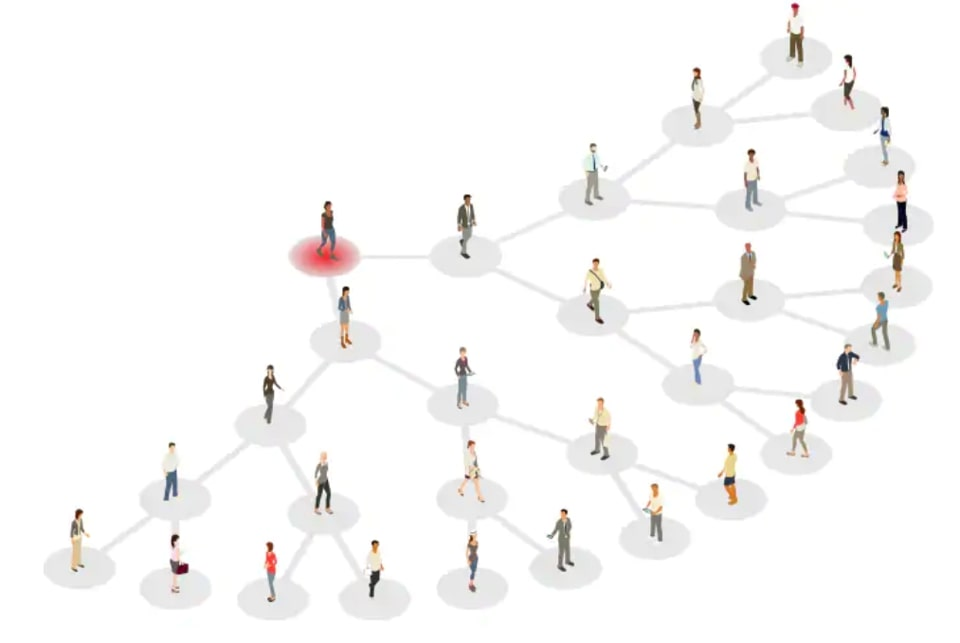
\includegraphics[height=5.3cm]{immagini/contacttracing}
  \captionof{figure}{Rappresentazione schematica del \textit{contact tracing}.}
  \caption*{\textbf{Fonte:} mashable.com}
\end{minipage} \\

Tra le aziende che si sono mobilitate per questa causa c'è anche Sync Lab, che ha avviato un suo progetto in tale ambito chiamato \textit{SyncTrace}. Questo sistema ha come scopo lo sviluppo di due prodotti differenti ma in relazione tra loro: un'applicazione di \textit{contact tracing} puro e un applicativo di gestione e organizzazione per i medici e per gli esercenti di attività commerciali. \\

Il \textbf{primo} applicativo, mostrato in \hyperref[img:synctraceandroid]{Figura 2.2}, è pensato per l'utilizzo da parte di tutta la popolazione e ha come unico scopo il tracciamento dei contatti delle persone infette; esso è in forma di applicazione per dispositivi mobili, quali \textit{smartphone} e \textit{tablet}, ed è pensato in modo da tracciare i contatti e i livelli di rischio di positività basandosi su parametri oggettivi come la vicinanza e il tempo di esposizione. \\

\begin{minipage}{\linewidth}
  \label{img:synctraceandroid}
  \centering
    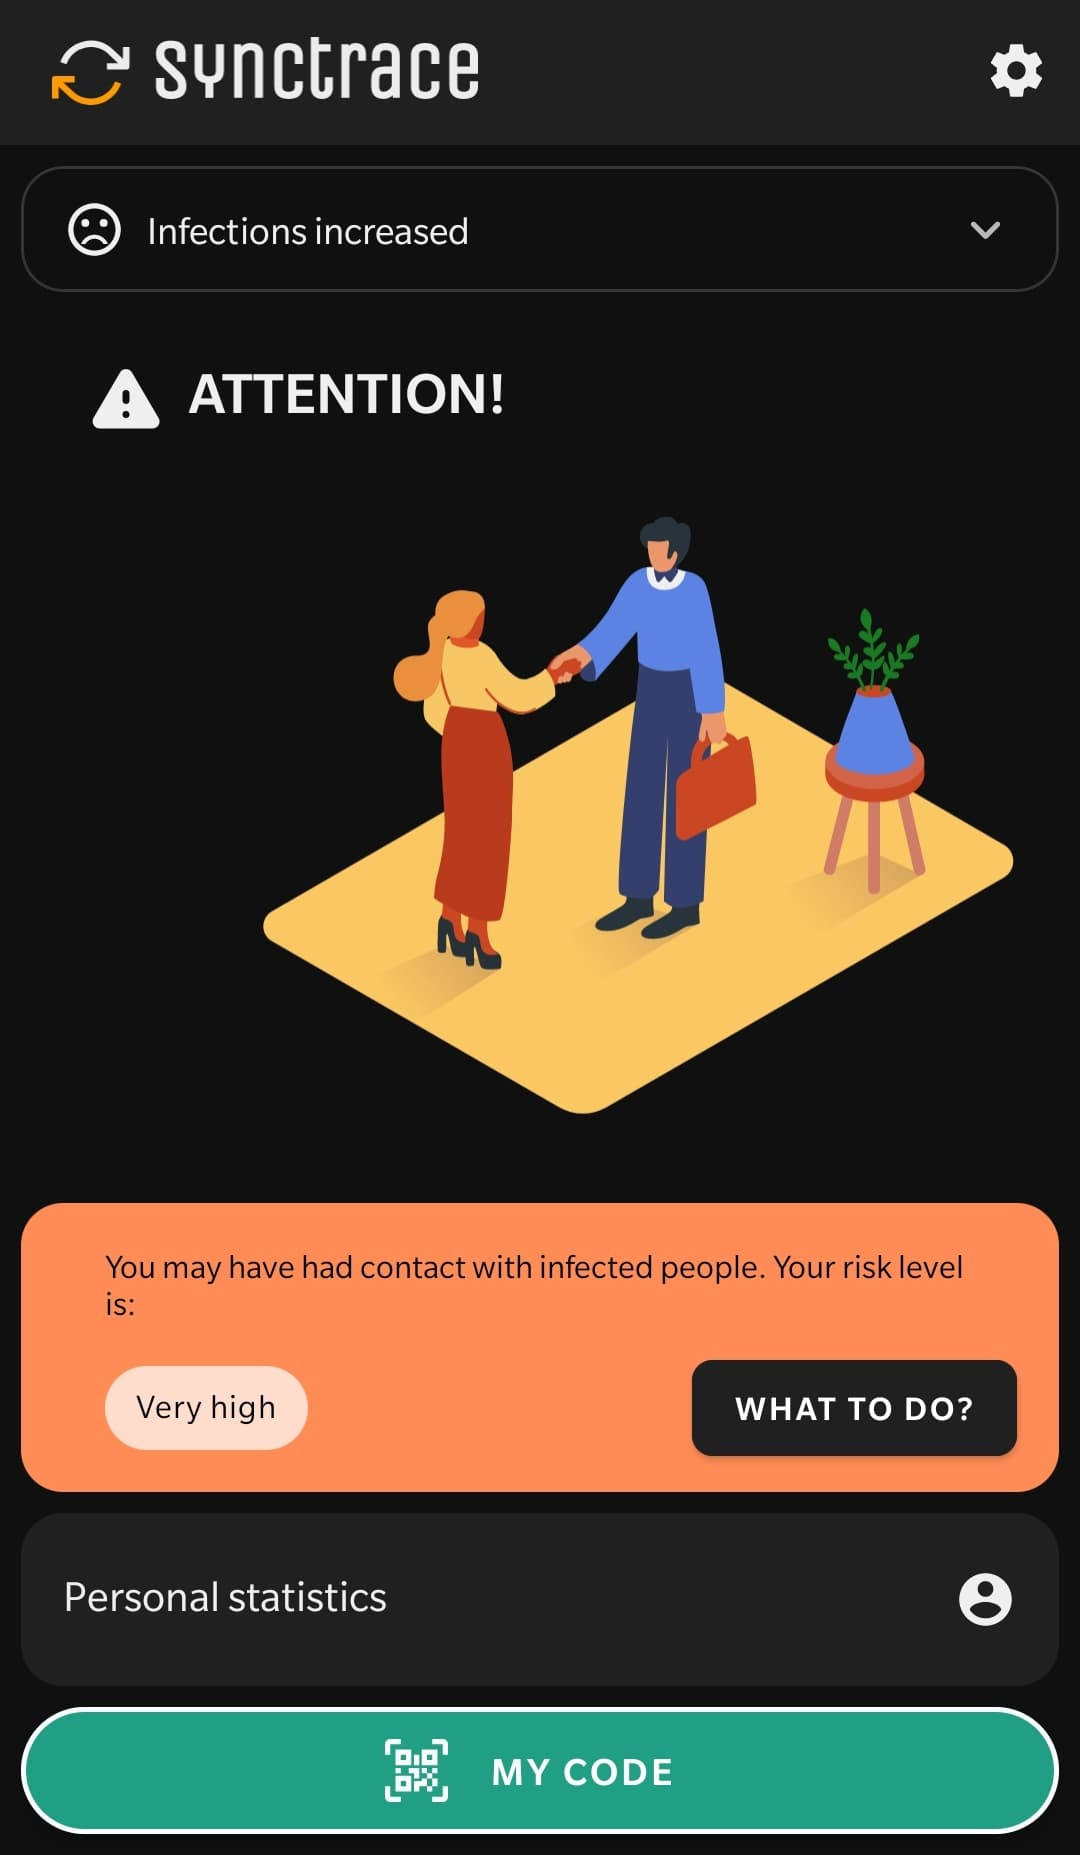
\includegraphics[height=7.8cm]{immagini/synctraceandroid}
  \captionof{figure}{Immagine di cattura di schermo iniziale dell'applicazione \textit{SyncTrace}.}
\end{minipage} \\

Il \textbf{secondo} applicativo, consistente in una \textit{web application} rappresentata in \hyperref[img:webapp]{Figura 2.3}, è pensato per fornire un'interfaccia di gestione del sistema ai medici e come applicazione di controllo per gli esercenti. Esso ha quindi un doppio utilizzo:
\begin{itemize}
  \item I \textbf{medici}, una volta identificati come tali, possono usarlo per registrare nuovi contatti infetti, eliminare i dati di eventuali pazienti non infetti e verificarne la presenza e/o il livello di rischio di contagio nel sistema condiviso;

  \item Gli \textbf{esercenti}, una volta registrati come tali, possono controllare l'eventuale positività o il livello di rischio di contagio dei clienti che accedono alle proprie attività. \\
\end{itemize}

\begin{minipage}{\linewidth}
  \label{img:webapp}
  \centering
    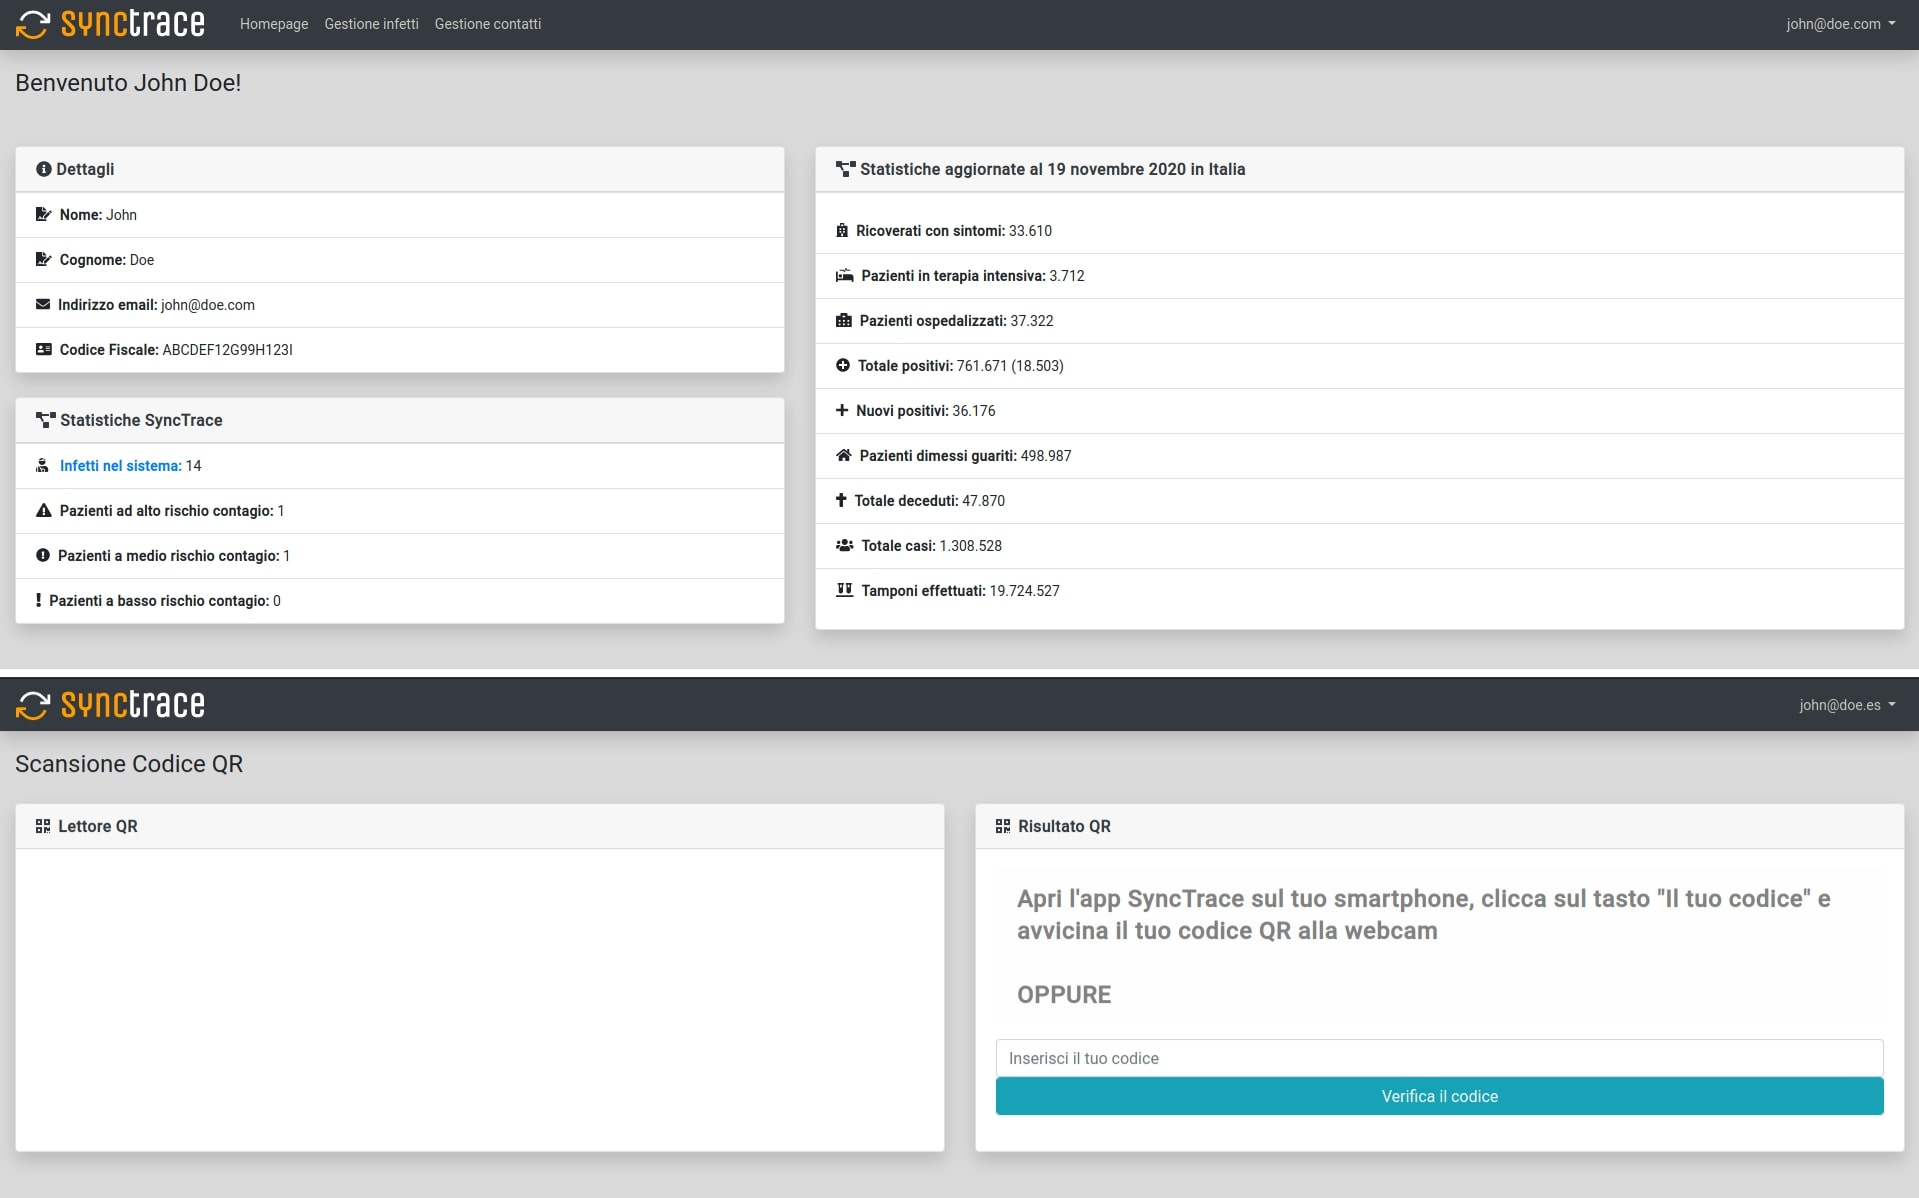
\includegraphics[height=7.2cm]{immagini/webapp}
  \captionof{figure}{Immagine di cattura di schermo iniziale della \textit{webapp} per, rispettivamente, medici ed esercenti.}
\end{minipage} \\

Il mio progetto di \textit{stage} si inserisce nel contesto di quest'ultimo applicativo descritto. Lo scopo principale del mio tirocinio è, infatti, effettuare il \textit{porting} dell'applicativo utilizzando il \textit{framework Ionic}\footcite{tec:ionic}, per poter riutilizzare parte della logica già sviluppata secondo il principio del \textit{write once, run anywhere}.

%**************************************************************

\section{Vincoli e obiettivi dello stage}

Prima di cominciare il tirocinio ho definito, insieme al tutor aziendale, gli obiettivi e i vincoli che il mio lavoro avrebbe dovuto rispettare. Questo ha portato alla stesura di un \textbf{piano di lavoro}, riportante lo scopo dello stage, i prodotti attesi, la pianificazione settimanale del lavoro e gli obiettivi del progetto; durante il progetto, però, questo piano di lavoro ha subito due modifiche per meglio adattarsi a esigenze personali e per occupare al meglio il tempo in termini di produttività.

\subsection{Vincoli temporali}

Lo \textit{stage} aveva una durata prevista di 8 settimane, di cui 7 da 40 ore l'una e l'ultima da 20 ore, per un totale di 300 ore. Come già detto, la maggior parte del progetto si è svolto in \textit{smart working}: ho quindi lavorato una media di 8 ore giornaliere da casa. \\
I giorni in cui mi sono recato in ufficio, generalmente il venerdì di ogni settimana, l'orario di lavoro è stato dalle 09.00 alle 18.00, con un'ora di pausa pranzo. Di seguito, in \hyperref[tab:attivita-settimanali]{Tabella 2.1}, riporto un riassunto delle attività svolte, divise per ore e settimane.

\begin{table}[h]
  \label{tab:attivita-settimanali}
  \begin{tabularx}{\textwidth}{|l|l|X|}
  \hline
  \textbf{Settimana}          & \textbf{Ore} & \textbf{Attività}         \\ \hline
  \multirow{3}{*}{\textit{1}} & 8            & \textbf{Formazione} sul linguaggio \textit{Java SE}  \\ \cline{2-3}
                              & 16           & \textbf{Formazione} sul linguaggio \textit{Java EE}  \\ \cline{2-3}
                              & 16           & \textbf{Formazione} sul \textit{framework Spring}    \\ \hline
  \textit{2}                  & 40           & \textbf{Formazione} sul \textit{framework Spring}                    \\ \hline
  \multirow{3}{*}{\textit{3}} & 24           & \textbf{Formazione} sul linguaggio \textit{JavaScript}                        \\ \cline{2-3}
                              & 8            & \textbf{Formazione} sul linguaggio \textit{TypeScript}                        \\ \cline{2-3}
                              & 8            & \textbf{Formazione} sul \textit{runtime NodeJS}                     \\ \hline
  \textit{4}                  & 40           & \textbf{Formazione} sul \textit{framework Angular}                   \\ \hline
  \multirow{3}{*}{\textit{5}} & 20           & \textbf{Formazione} sul \textit{framework Ionic} e su quanto fatto nel progetto precedente \\ \cline{2-3}
                              & 4            & \textbf{Configurazione} dell'ambiente di produzione            \\ \cline{2-3}
                              & 16           & \textbf{Codifica} delle maschere previste dal progetto  \\ \hline
  \multirow{2}{*}{\textit{6}} & 24           & \textbf{Codifica} delle maschere previste dal progetto  \\ \cline{2-3}
                              & 16           & \textbf{Configurazione} del \textit{server} di \textit{back-end} tramite containerizzazione con piattaforma \textit{Docker}                   \\ \hline
  \textit{7}                  & 8            & \textbf{Configurazione} del \textit{server} di \textit{back-end} tramite containerizzazione con piattaforma \textit{Docker}           \\ \hline
  \multirow{2}{*}{\textit{8}} & 16           & \textbf{Codifica} delle ultime maschere e di componenti aggiuntive           \\ \cline{2-3}
                              & 24           & \textbf{Verifica} del codice scritto                  \\ \hline
  \multirow{3}{*}{\textit{9}} & 8            & \textbf{Collaudo} dell'applicativo prodotto                  \\ \cline{2-3}
                              & 24           & \textbf{Documentazione} dell'intero progetto            \\ \cline{2-3}
                              & 8            & \textbf{Codifica e verifica} di ultimi \textit{fix} a \textit{bug} trovati tramite il collaudo                \\ \hline
  \end{tabularx}
  \caption{Suddivisione settimanale delle attività}
\end{table}

\subsection{Vincoli organizzativi}

Prima di cominciare lo \textit{stage} ho inoltre pattuito i vincoli organizzativi con il tutor aziendale. Come già detto, per quanto riguarda questo frangente è stato deciso di lavorare in \textit{smart working} per la maggior parte della durata del progetto; abbiamo inoltre deciso di incontrarci periodicamente, solitamente il venerdì, per fare il punto della situazione e potermi allineare con il tutor aziendale. \\
Ho rendicontato il lavoro che ho effettuato, sia in remoto che in presenza, in un foglio di calcolo online riportante la data, le attività svolte in tale data e l'approvazione o meno da parte del tutor aziendale; ho aggiornato questo documento quotidianamente, e settimanalmente ho ricevuto il \textit{feedback} da parte del tutor. In \hyperref[img:drive]{Figura 2.4} riporto una porzione di tale documento. \newpage

\begin{minipage}{\linewidth}
  \label{img:drive}
  \centering
    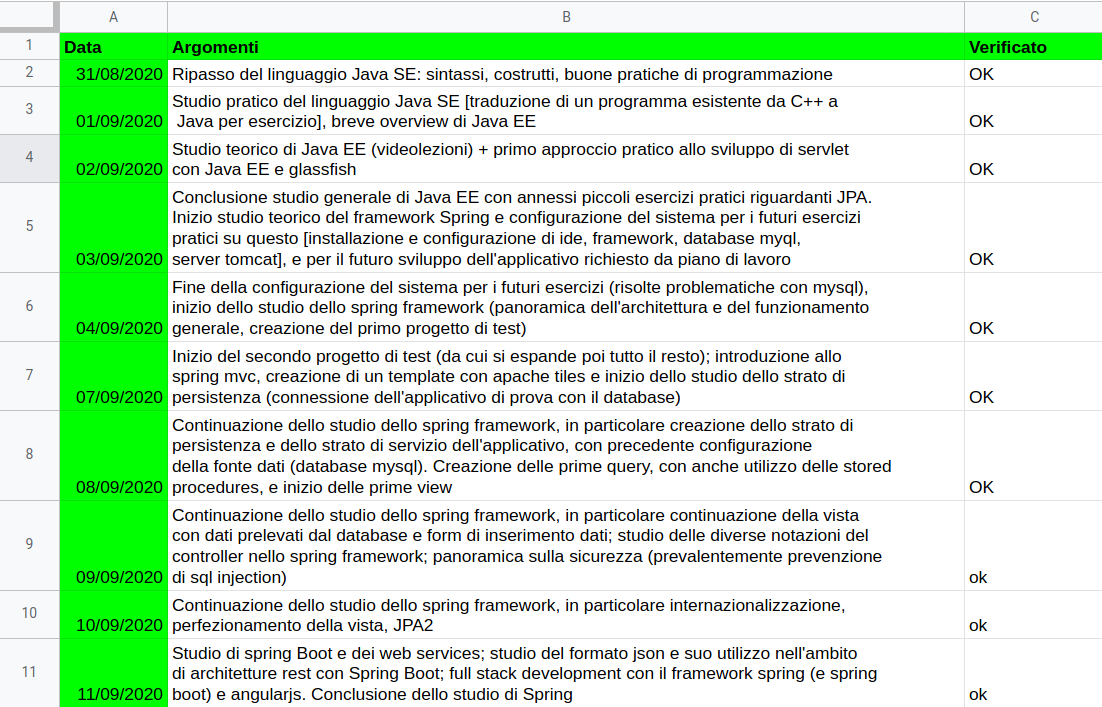
\includegraphics[height=7.5cm]{immagini/drive}
  \captionof{figure}{Porzione del registro delle attività.}
\end{minipage} \\

Per quanto riguarda il salvataggio e il versionamento del codice e della documentazione prodotti, inoltre, ho fatto uso della \textit{repository GitLab} aziendale.

\subsection{Vincoli tecnologici}

Per quanto riguarda i vincoli tecnologici, posso dire di essere stato abbastanza libero nella scelta di quali strumenti utilizzare; i vincoli a cui sono sottostato sono quindi stati decisi principalmente da me, in accordo con il tutor aziendale, come riporto di seguito.

\subsubsection*{Sistema operativo}

Essendo il prodotto a cui ho lavorato non coperto da segreto industriale, ho svolto l'intero progetto sulla mia macchina senza bisogno di software esterni per rispettare le norme di sicurezza aziendali. Il sistema operativo che ho utilizzato per lo sviluppo è stato \textit{GNU/Linux}, in particolare la distribuzione \textit{Arch Linux} a 64 bit.

\subsubsection*{PostgreSQL}
Sebbene il mio lavoro non comprendesse l'utilizzo diretto di un \textit{database}, la componente \textit{back-end} dell'applicativo fa uso del \textit{database} relazionale \textit{PostgreSQL}\footcite{tec:postgres}; ho avuto modo di utilizzare questa tecnologia durante il processo di collaudo, per verificare che i dati inseriti dall'applicazione venissero correttamente immagazzinati dal \textit{database}.

\subsubsection*{Docker}
Per effettuare il \textit{deployment} della componente \textit{back-end} dell'applicativo, necessaria al processo di collaudo su dispositivo mobile, ho fatto uso dello strumento di containerizzazione \textit{Docker}\footcite{tec:docker}. Questo mi ha permesso di rendere la suddetta componente installabile facilmente su qualsiasi sistema.

\subsubsection*{Android Studio}
Per effettuare il collaudo di quanto sviluppato su dispositivo mobile, sono stato vincolato all'ambiente di sviluppo integrato \textit{Android Studio}, fornito gratuitamente dall'azienda \textit{JetBrains}, per la compilazione dell'applicazione per dispositivi \textit{Android}; in accoppiata a questo ho utilizzato il \textit{tool ADB} (\textit{Android Debug Bridge}) per l'installazione dell'applicazione sul dispositivo.

\subsubsection*{Documentazione}
Per quanto riguarda la documentazione, su consiglio del mio tutor aziendale la mia scelta è ricaduta sul \textit{tool Compodoc}\footcite{tec:compodoc}, uno strumento simile a \textit{Javadoc} per applicazioni sviluppate tramite il \textit{framework Angular}; questo strumento ha permesso la generazione automatica di documentazione a partire da commenti strutturati al codice.

\subsection{Obiettivi}

Insieme al tutor aziendale ho delineato gli obiettivi dello \textit{stage} e li ho riportati in un piano di lavoro validato dal tutor interno, il prof. Tullio Vardanega. \\
Ogni obiettivo possiede un nome formato nel seguente modo:
\begin{center}
  \centering
  \texttt{O-[tipologia][numero]}
\end{center} dove:
\begin{itemize}
  \item \texttt{[tipologia]} indica la tipologia di obiettivo. Questa può essere:
  \begin{itemize}
    \item \texttt{O}: obbligatorio, ossia un obiettivo vincolante e necessario da soddisfare;
    \item \texttt{D}: desiderabile, ossia un obiettivo non vincolante ma dal riconoscibile valore aggiunto;
    \item \texttt{F}: facoltativo, ossia un obiettivo non vincolante e rappresentante un valore aggiunto non competitivo.
  \end{itemize}
  \item \texttt{[numero]} consiste in un numero, progressivo per ogni tipologia.
\end{itemize}

Di seguito riporto, in \hyperref[tab:obiettivi-originali]{Tabella 2.2}, gli obiettivi inizialmente individuati.
\newpage

\begin{table}[h]
  \label{tab:obiettivi-originali}
\begin{tabularx}{\textwidth}{|l|X|}
\hline
\textbf{Obiettivo}           & \textbf{Descrizione}                                                                                                                          \\ \hline
\texttt{O-O1} & Acquisizione delle competenze su linguaggi di programmazione, \textit{framework} e strumenti di supporto                                              \\ \hline
\texttt{O-O2} & Capacità di raggiungere gli obiettivi richiesti in autonomia seguendo il cronoprogramma                                                       \\ \hline
\texttt{O-O3} & Portare a termine le implementazioni previste con una percentuale di superamento pari all'80\%                                                \\ \hline
\texttt{O-D1} & Portare a termine le implementazioni previste con una percentuale di superamento pari al 100\%                                                \\ \hline
\texttt{O-F1} & Dare un contributo importante nelle fasi di progettazione delle maschere con l'obiettivo di realizzare una app usabile, \textit{responsive} e \textit{adaptive} \\ \hline
\texttt{O-F2} & Implementare la lettura del \textit{QR Code} direttamente dalla fotocamera dello \textit{smartphone}, evitando quindi inserimenti manuali                       \\ \hline
\end{tabularx}
\caption{Obiettivi di progetto originali.}
\end{table}

In corso di progetto il piano di lavoro è stato rimodulato, in quanto ho svolto parte del lavoro in un tempo minore del previsto; ai precedenti obiettivi si è quindi aggiunto l'obiettivo che riporto in \hyperref[tab:ulteriore-obiettivo]{Tabella 2.3}.

\begin{table}[h]
  \label{tab:ulteriore-obiettivo}
\begin{tabularx}{\textwidth}{|l|X|}
\hline
\textbf{Obiettivo}           & \textbf{Descrizione}                                                                                                                          \\ \hline
\texttt{O-D2} & Containerizzazione della componente \textit{back-end} del progetto \textit{SyncTrace}                                              \\ \hline
\end{tabularx}
\caption{Ulteriore obiettivo, aggiunto in corso di progetto.}
\end{table}

Il piano di lavoro identifica inoltre i prodotti attesi, cioè:
\begin{itemize}
  \item Un \textbf{documento tecnico} che descriva le maschere utilizzate;
  \item Il \textbf{codice} rilasciato sul \textit{repository} indicato dall'azienda.
\end{itemize}

%**************************************************************

\section{Motivazione della scelta}

Sono venuto a conoscenza di Sync Lab durante l'evento \textbf{StageIT 2020}. Questo evento, organizzato dal prof. Tullio Vardanega dell'\textit{Università degli Studi di Padova} in collaborazione con l'associazione di imprenditori \textit{Assindustria Venetocentro}, è un'occasione in cui gli studenti di diverse facoltà dell'università di Padova vengono messi in contatto con le aziende presenti sul territorio. \\
L'evento viene organizzato annualmente; quest'anno, però, a causa dell'emergenza sanitaria non si è potuto svolgere in presenza. Nonostante questo, l'adesione da parte delle aziende e degli studenti è stato comunque soddisfacente, anche grazie al fatto che, seguendo gli incontri con le aziende per via telematica, è stato possibile contattarne più di una contemporaneamente. \\

Durante l'evento \textit{StageIT} ho avuto occasione di parlare con i rappresentanti di quattro aziende operanti nel comune di Padova, tra cui l'ing. Fabio Pallaro di Sync Lab. \\
Gli ambiti di \textit{stage} a cui ero interessato erano principalmente tre: sviluppo software \textit{mobile}, \textit{data science} e \textit{cybersecurity}. Uno dei motivi per cui ho optato per Sync Lab come azienda è stato che l'ing. Pallaro mi ha offerto due diversi ambiti di \textit{stage}: uno riguardante lo sviluppo di un'applicazione per dispositivi mobili tramite \textit{framework Ionic}, e uno riguardante l'aspetto di sicurezza dei prodotti che l'azienda stava e avrebbe sviluppato con altri tirocinanti, entrambi ambiti a cui ero particolarmente interessato. L'azienda, inoltre, mi è sembrata molto attenta agli studenti interessati a un tirocinio presso di essa, segno a mia opinione di serietà, professionalità e apertura a nuove esperienze. \\
Per quanto riguarda il progetto, ho infine optato per lo sviluppo di un applicativo mobile per svariati motivi, anzitutto l'ambito: la tematica del \textit{contact tracing} mi è infatti fin da subito interessata per l'utilità che può avere in situazioni come quella attuale. Oltre a questo, ho trovato che le tecnologie che sarei poi andato ad utilizzare fossero interessanti da un punto di vista personale e, soprattutto, professionale: i linguaggi \textit{JavaScript} e \textit{TypeScript} e i \textit{framework} web e \textit{mobile} come \textit{Angular} e \textit{Ionic}, infatti, sono utilizzati sempre di più frequentemente dalle aziende operanti nel settore \textit{IT}.

%**************************************************************

\section{Formazione}

Ho dedicato il primo mese del mio tirocinio allo studio e all'approfondimento di tutte le conoscenze che mi sarebbero servite, o mi sarebbero state utili, a sviluppare il progetto di \textit{stage} vero e proprio. Gli \textbf{strumenti} che ho utilizzato a tale scopo sono molteplici: anzitutto, ho fatto uso della piattaforma \textit{Udemy} per acquisire le informazioni teoriche riguardanti le tecnologie oggetto di studio; a questo ho associato anche l'utilizzo della piattaforma \textit{YouTube}, sulla quale ho trovato svariati video di particolare utilità. Per quanto riguarda gli esercizi pratici, invece, ho fatto uso sia della piattaforma \textit{Udemy} che di \textit{tool} per l'esercitazione, quali ad esempio il pacchetto \textit{npm "LearnYouNode"}\footcite{tec:learnyounode} per quanto riguarda lo studio del \textit{runtime NodeJS}. \\

\subsection{Tecnologie}
Ho cominciato lo studio delle tecnologie con il linguaggio di programmazione \textbf{Java}, del quale ho appreso principalmente la sintassi, i costrutti di base e, soprattutto, l'implementazione di \textit{servlet} e le \textit{JPA} (\textit{Java Persistence API}) del linguaggio \textit{Java Enterprise Edition}. Sebbene il mio progetto non prevedesse lo sviluppo in codice \textit{Java}, la componente \textit{back-end} del prodotto cui il mio progetto appartiene è scritto con questo linguaggio in accoppiata al \textit{framework Spring}; ho quindi ritenuto opportuno, insieme al tutor aziendale, approfondire questo argomento per poter comprendere almeno a grandi linee il funzionamento del \textit{back-end}. Successivamente ho quindi studiato il \textit{framework} \textbf{Spring}: di questo ho appreso a grandi linee il funzionamento generale, comprendente i diversi strati da cui è composto un applicativo sviluppato con questa tecnologia (\textit{database}, persistenza, \textit{business} e presentazione). \\
Una volta terminato lo studio delle tecnologie riguardanti la componente \textit{back-end} del prodotto, sono passato allo studio di quelle riguardanti la componente \textit{front-end}. Ho quindi cominciato con lo studio di \textbf{JavaScript}, linguaggio del quale avevo già delle conoscenze abbastanza radicate; di questo ho quindi approfondito aspetti avanzati, quali \textit{promise}, \textit{fetch api} e le funzioni asincrone. Sebbene anche questo linguaggio non fosse previsto dal mio progetto, è stato comunque utile da studiare come base per lo studio di \textbf{TypeScript}, che è stato quello principalmente utilizzato per lo sviluppo dell'applicativo del mio progetto. \\
Una volta concluso lo studio di questi linguaggi di programmazione ho approfondito i \textit{framework} che li utilizzano nel contesto del mio progetto di \textit{stage}. Per primo ho studiato \textbf{Angular}, che è la tecnologia utilizzata per lo sviluppo dell'applicativo di cui il mio progetto prevedeva il \textit{porting}; è stato quindi necessario studiarlo per capire al meglio come fosse strutturato tale applicativo. Ho infine approfondito il \textit{framework} \textbf{Ionic} che è stato quello che più ho utilizzato per lo sviluppo. \\

Per completare le mie conoscenze in ambito \textit{back-end JavaScript}, inoltre, ho studiato il \textit{runtime} \textbf{NodeJS}. Nessun componente del prodotto a cui il mio progetto appartiene è sviluppato interamente con \textit{NodeJS}; alcune componenti di esso vengono utilizzate, però, per la gestione del collegamento tra la componente \textit{front-end} e quella \textit{back-end} dell'applicativo di cui ho eseguito il \textit{porting}. \\
Ho infine approfondito \textbf{Docker}, piattaforma che automatizza il \textit{deployment} di applicazioni all'interno di macchine virtuali \textit{linux} minimali. Ho approfondito questo argomento a sviluppo già cominciato, poiché per il processo di collaudo si è reso necessario per me avere la componente \textit{back-end} del prodotto su un \textit{server} accessibile via \textit{http}, e mi è stato proposto di containerizzare tale componente per poter effettuare un \textit{deployment} più efficiente. In \hyperref[img:tecnologie]{Figura 2.5} ho riportato uno schema che mostra come le diverse tecnologie interagiscono tra loro nel caso del progetto oggetto del mio \textit{stage}. \\

\begin{minipage}{\linewidth}
  \label{img:tecnologie}
  \centering
    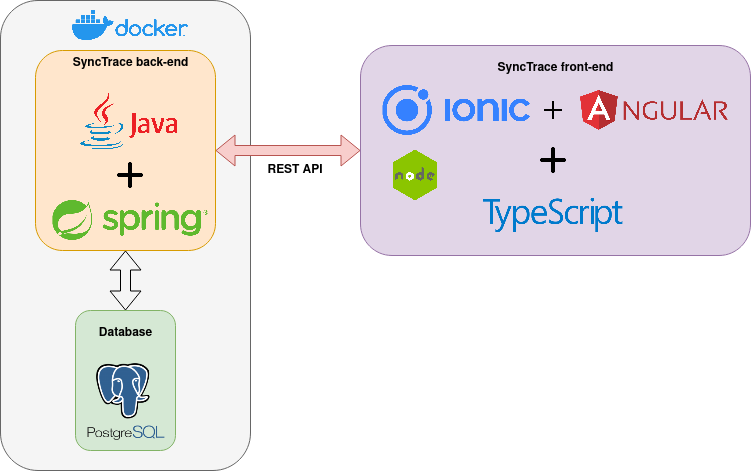
\includegraphics[height=5.2cm]{immagini/tecnologie}
  \captionof{figure}{Schema rappresentante le relazioni che sussistono tra le tecnologie descritte in SyncTrace.}
\end{minipage}

\subsection{Progetto}

Come precedentemente riportato, il mio progetto si è concretizzato nell'effettuare il \textit{porting} di una \textit{web application} su dispositivi mobili tramite il \textit{framework Ionic}. L'applicazione web, consistente in una \textit{single page application} sviluppata in \textit{TypeScript} tramite il \textit{framework Angular}, offre le stesse funzionalità dell'applicativo sviluppato da me; molte di queste, però, non sono traslabili direttamente su \textit{mobile}, poiché consistenti di elementi non nativi dei sistemi operativi mobili. Esempio di ciò sono sia piccolezze estetiche, quali ad esempio i bottoni, i \textit{form} e gli \textit{alert}, che l'utilizzo delle risorse hardware del sistema, quali ad esempio la fotocamera, i bottoni fisici e gli strumenti di misura come l'accelerometro. Ho quindi effettuato anche uno studio su quanti e quali componenti software avrei dovuto cambiare per sviluppare correttamente il mio prodotto.

%**************************************************************
